\documentclass{article}

\usepackage{amsmath} 
\usepackage{graphicx}
\usepackage{amsfonts}
\usepackage{array}


\begin{document}

\title{Catam 16.5 Permutation Groups}
\date{September 2023}

\section{Groups and the Stripping Algorithm of Sims}
\subsection{Permutations}

To define a group element $g$, of the symmetric group $S_n$ behaves it suffices
to consider its behaviour on the set $X = \{1, 2, \dots n\}$. As the language
I will be using for this project is python, the code will take $X = \{0, 1, \dots n-1\}$, however there is no substantial difference between these paradigms

\vspace*{5mm}

Now we can define in terms of an array data structure how a permutation will be defined.
Simply considering the bijection $g : X \rightarrow X$. If we define an array of size $n$ and fill the entries such that
$g[i] = g(i)$ we encapsulate all the needed information.

\subsubsection{Question 1}

Question 1 asks for a program to compute the inverse and product of two permutations which under the current paradigm is very easy.
Firstly let us consider inverses. Let $h = g^{-1}$

$$h(g(i)) = i \implies h[g[i]] = i$$

Now as $g$ is a bijection we have fully specified $h$. For products it is just as simple. Let $h = fg$

$$h(i) = f(g(i)) \implies h[i] = f[g[i]]$$

The only issue that could arise is from the ordering of $f$ and $g$, due to $S_n$ being non-abelian, however if we keep with convention of left and right multiplication then there will be no issue.
The code for this question can be found in the "Code" Section. Here are some examples of computations with these algorithms.

	[[LOL NO DO IT LATER]]

\vspace*{5mm}

Considering complexity of our algorithms it is clear to see that they are both $O(n)$ noting that we simply iterate through each $i$ and assign one index a value each time.

\subsection{Stripping Algorithm}

\subsubsection{Question 2}

Let the entries of the stripping algorithm, $\pi_1 \dots \pi_k$ generate $G$.
Let us assume that by the time we reach $\pi_i$, the current output, $\rho_1 \dots \rho_l$ can generate $\pi_1 \dots \pi_{i-1}$
Now supposing we combine some modifications as per the algorithm to fix any amount of entries, we may write $g = \rho^{-1}\pi_i$ with $\rho \in\ <\rho_1 \dots \rho_l>$
Now if we terminate $g$ as the identity then it is clear that $\pi_i$ is generated by the output. If we do not terminate on the identity
it follows that $g$ is added to the output and so clearly $\pi_i$ is still generated by the output at that point. Finally by induction it is clear that the output generates $G$.

\vspace*{5mm}

Let us consider the nature of the algorithm. Suppose we reach the $i$th row, that is $1 \dots i-1$ are fixed. We can have at most $n-i$ non-trivial entries,
this is from the choice of $g(i)$ given $g(1) = 1, \dots g(i-1) = i-1$. Now consider each possible entry is filled, then it would be impossible to add another element to the array.
This is because we may always fix 1 in any circumstance, then we can always fix 2 and so on. We may always revert back to the identity. This gives us a natural upper bound of:

$$\sum_{i = 1}^{n}(n-i) = n^2 - \frac{1}{2}n(n+1) = \frac{1}{2}n(n-1)$$

\begin{table}[h!]
	\centering
	\begin{tabular}{ |c|c|c|c c c|c| }
		\hline
		N/A      & $\rho_1$ & $\rho_4$ & $\rho_7$ & $\dots$  &     & $\rho_3$ \\ \hline
		N/A      & N/A      & $\rho_2$ & $\rho_9$ & $\dots$  &     &          \\ \hline
		N/A      & N/A      & N/A      &          & $\dots$  &     & $\rho_6$ \\ \hline
		N/A      & N/A      & N/A      & N/A      & $\dots$  &     &          \\
		$\vdots$ & $\vdots$ & $\vdots$ & $\vdots$ & $\ddots$ &     &          \\
		N/A      & N/A      & N/A      & N/A      &          & N/A & $\rho_8$ \\ \hline
		N/A      & N/A      & N/A      & N/A      &          & N/A & N/A      \\ \hline
	\end{tabular}
\end{table}

\subsubsection{Question 3}
Question 3 asks for a program to find the new generators according to this procedure. It can be found in the "Code" section of the project.
I will now provide a few examples.

	[[LOL NO DO IT LATER]]

\section{Orbit Stabilizer and Schreier's Theorem}
\subsection{Orbit Stabilizer Theorem}
Consider the map:

$$\Phi: G/G_{\alpha} \rightarrow Orb_{G}(\alpha)\ \ \ \ \Phi(gG_{\alpha}) = g\alpha$$

To prove this is a bijection we must prove, it is well defined, injective and surjective.
To prove it is well defined and injective:

$$gG_\alpha = hG_\alpha \iff g^{-1}h \in G_\alpha \iff g^{-1}h\alpha = \alpha \iff h\alpha = g\alpha$$

Surjectivity follows from if $\beta \in Orb_G(\alpha) \implies \exists g\ g\alpha = \beta$ so the coset $gG_\alpha$ is the natural choice.

\vspace*{5mm}

The immediate consequence of this is the Orbit Stabilizer Theorem which states for $G$ finite $|G| = |G_\alpha| |Orb_G(\alpha)|$. To prove we use the bijection we constructed
and Lagrange's theorem.
$|Orb_G(\alpha)| = |G/G_\alpha| = |G: G_\alpha| = |G| / |G_\alpha|$.

\subsubsection{Question 5}
Question 5 asks for a program to find the orbit and witness of some value $\alpha$ for a group generated by given permutations.
The code can be found in the "Code" section. Here follows a few examples.

	[[LOL NO DO IT LATER]]

The algorithm is fairly simple. We first note that we need only consider the action of generators as all other elements may be constructed from them.
We iterate through each generator and if say $g\alpha = \beta$ then we store $g$ in the position $\beta$ of an array of size $n$. Then we may repeat the process iterating the generators instead on $\beta$ this time and storing $hg$ for $h$ sending $\beta$ to $\gamma$.
We continue searching until we cannot expand the size of the orbit anymore. Simply storing some element constructed from generators which serves as a witness.
Then returning this array yields all the information needed.

\subsection{Schreier's Theorem}

[[Mafs]]

\subsubsection{Question 7}
Question 7 asks for a program to find generators of a stabilizer.
The code can be found in the "Code" section. Here follows a few example computations.

	[[LOL NO DO IT LATER]]

	[[This algorithm has a bad time complexity like really bad but we move.]]



\subsubsection{Question 8}
Question 8 asks for a program to find the order of a group $G$.
We use the code created in question 7 to find the generators of stabilizers.
Then we fix each element of $X$ in turn finding each successive stabilizer and orbit as we go.
Then we finally use the Orbit Stabilizer theorem to find the final result.

\vspace{5mm}

We let $G = G_0$ and consider $G_i$ to be the stabilizer of $G_{i-1}$ fixing $i$. Then it follows that
$$G \geq G_1 \geq \dots \geq G_n \cong \{ e \}$$

The orbit stabilizer theorem then gives by induction:

$$|G_{i}| = \prod_{j=i+1}^{n} |Orb_{G_{j-1}}(j)|$$

$$|G| = \prod_{j = 1}^{n} |Orb_{G_{j-1}}(j)|$$

\vspace{5mm}

The code can be found in the "Code" section. Here follows a few example computations.

	[[LOL NO DO IT LATER]]

	[[Prolly wanna reword this I suppose I am kinda >:| ]]



\subsubsection{Question 9}
$P_n$ is the probability that two elements of $S_n$ generates $S_n$. We know, from IA, that the following elements expressed in cycle notation $(1 2), (1 2 3 \dots n)$ generate $S_n$ so $P_n > 0$.

\vspace*{5mm}

Consider $A_n$. The probability that both elements chosen lie in $A_n$ is $\frac{1}{4}$ and hence we must have $P_n \leq \frac{3}{4}$ due to $A_n$ being a subgroup.

\vspace*{5mm}

We may tabulate results for small $n$ by simply exhausting every option. A program has been written to run this computation and can be found in the "Code" section.


\begin{table}[h!]
	\centering
	\begin{tabular}{ |c|c|c|c| }
		\hline
		$n$   & $2$    & $3$   & $4$     \\ \hline
		$P_n$ & $0.75$ & $0.5$ & $0.375$ \\ \hline
	\end{tabular}
	\caption{Table of $P_n$ for $n$ small.}
\end{table}


To generate a random permutation efficiently is very simple. First let us begin with an array of numbers $A = [1, \dots n]$. We generate a random number, $k$, between $1$ and the size of the array and define $g[1] = k$.
Now we remove $k$ from $A$ and iterate the process with $g[2] \dots g[n]$ until $A$ has no more elements. Clearly we will have exhausted all the numbers $1$ to $n$ without repeats and no significant inefficiencies.

\vspace{5mm}

We may now use this to calculate approximations for $P_n$ by generating a few pairs at each $n$ and running the algorithm to compute the order of the group generated. Then we can compare the order against $n!$ to see if is indeed $S_n$. Some results are tabulated and graphed below.

\clearpage

\begin{table}[h!]
	\centering
	\begin{tabular}{ |c|cccccccc| }
		\hline
		$n$   & $5$   & $6$    & $7$   & $8$    & $9$    & $10$   & $11$   & $12$   \\ \hline
		$P_n$ & $0.5$ & $0.42$ & $0.6$ & $0.65$ & $0.61$ & $0.64$ & $0.71$ & $0.65$ \\ \hline
	\end{tabular}
	\caption{Approximations of $P_n$}
\end{table}

\begin{figure}[ht!]
	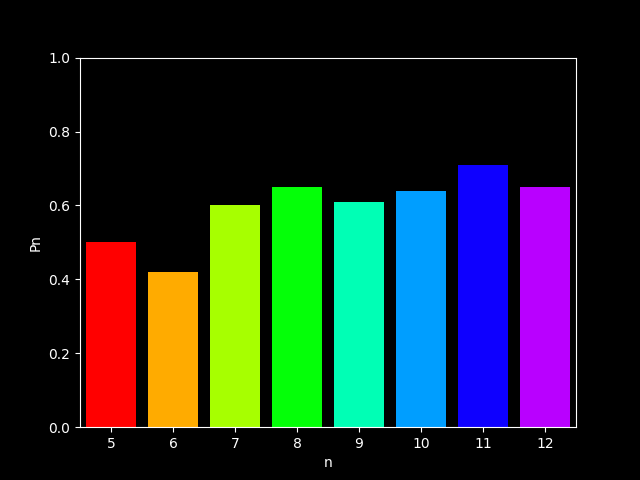
\includegraphics[width=\textwidth]{PnRainbow.png}
	\caption{Bar chart of $P_n$ approximations against $n$}
\end{figure}

We can see that perhaps contrary to intuition that $P_n$ does not go to $0$ but instead appears to increase. We note from an earlier discussion that $0.75$ is the probability that the group generated will not be a subgroup of $A_n$.
This then lends itself to the idea that in the long run, the probability that we generate either $S_n$ approaches $0.75$ exactly.

\end{document}